\documentclass[11pt]{article}
\usepackage{tdoc}
\usepackage{graphicx}
\usepackage{apacite}

% \draftfalse

\title{Sayram 2D: Numerical Algorithm}
\author{Xin Tao}

\begin{document}
\maketitle

\section{The 2D diffusion equation to be solved}
Sayram 2D aims to solve the 2D diffusion equation with a loss (or source term)
in the following form:
\begin{align}
   \frac{\partial f}{\partial t} = \frac{1}{G} \frac{\partial }{\partial Q_{i}}\left(G D_{Q_{i}Q_{j}}\frac{\partial f}{\partial Q_{j}}\right) - \frac{f}{\tau}. 
\end{align}
Equivalently,
\begin{align}
  \frac{\partial f}{\partial t} = \frac{1}{G}\nabla \cdot(\Lambda \cdot \nabla f) - \frac{f}{\tau}.
  \label{eq:general_2d_eq}
\end{align}
where 
\begin{align}
  \Lambda = \begin{bmatrix}
    GD_{Q_1Q_1} & GD_{Q_1Q_2} \\
    GD_{Q_1Q_2} & GD_{Q_2Q_2}
  \end{bmatrix}
\end{align}
is the diffusion tensor. The equation is subject to the following Dirichlet
($\Gamma_{D}$) and Neumann ($\Gamma_{N}$) boundary conditions:
\begin{align}
  f &= g_{D}, \quad \text{on } \Gamma_{D}, \\ 
  q_{N} &= \boldsymbol{n}\cdot \left(-\Lambda \cdot \nabla f\right), \quad \text{on } \Gamma_{N}.
\end{align}
The $q_{N}$ is the flux satisfying $q_{N} \leq 0$. Here $G > 0$ is the
Jacobian of the coordinate transformation, the $D_{Q_{i}Q_{j}}$ are diffusion
coefficients that may depend on time, and $\tau$ characterizes loss or
source. The $f/\tau$ term can be easily handled, and we will mainly deal with
the negative solution problem caused by the mixed diffusion coefficients using a
positivity-preserving finite volume method of \citeA{Gao2015}.

\section{A positivity-preserving finite volume method}
The PPFV method was developed by \citeA{Gao2015} and is reviewed here. Denoting the value of $f$ at cell $K$ as $f_{K}$, the basic principle of constructing the PPFV method is to write the equation to obtain $f_{K}(t+\Delta t)$ from $f(t)$ as follows:
\begin{align}
  \label{eq:appendix_convex}
  f_K(t+\Delta t) = \sum_{i}\alpha_i f_{K, i}(t),
\end{align}
where $f_{K,i}$ is the value of $f$ of the $i_{\text{th}}$ cell that contributes to updating the value of $f_{K}$. Note that this summation may also include $f_{K}$ itself. If all coefficients ($\alpha_{i}$'s) satisfy $\alpha_i \ge 0 $, and $f_{K,i}(t) \geq 0$, then the above equation guarantees that $f_{K}(t+\Delta t) \geq 0$. Clearly, for the radiation belt diffusion problem, the initial phase space density for every cell is non-negative. This illustrates the positivity principle; the method below achieves it through an $M$-matrix.

\begin{figure}[h]
  \centering
  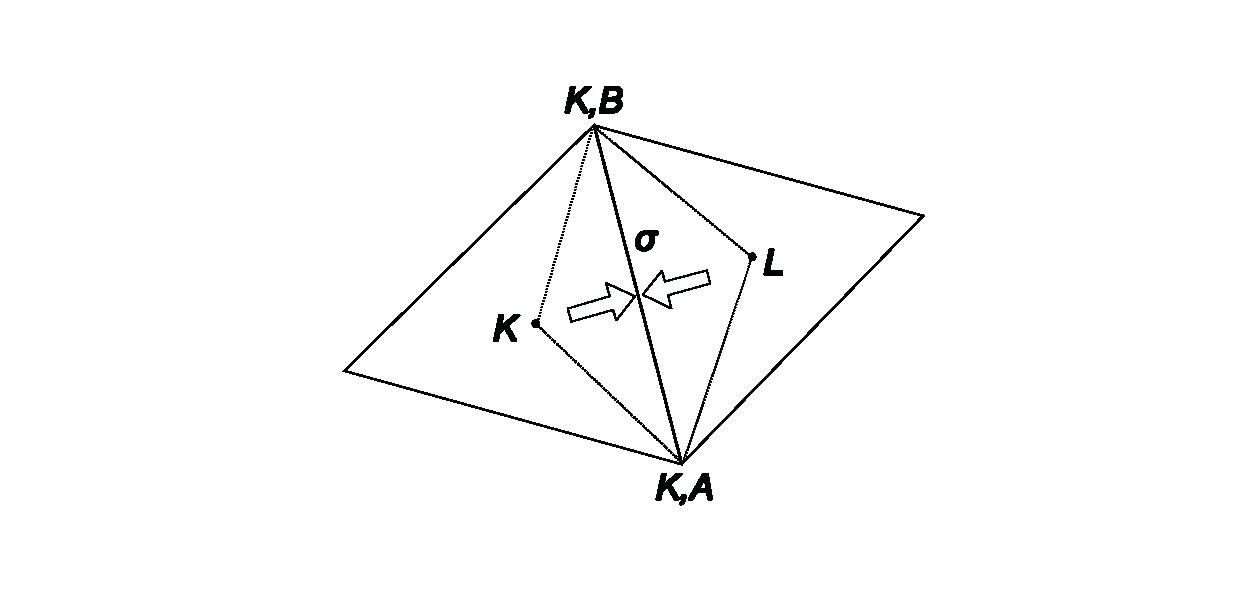
\includegraphics[width=\textwidth, keepaspectratio]{NTPFA_one_sided_flux}
  \caption{\label{fig:NTPFA_one_sided_flux}Illustration of the Nonlinear Two-Point Flux Approximation (NTPFA). We first construct a one-sided flux, from cell center $K$ to edge $\sigma$, using only values of $f_K$, $f_{K,A}$, $f_{K,B}$. This process is then repeated for the cell $L$. The flux used in the PPFV method to update $f_{K}$ or $f_{L}$ is derived using the one-sided fluxes.}
\end{figure}

We consider the diffusion equation part of Equation \eqref{eq:general_2d_eq}: 
\begin{align}
  \label{eq:appendix_diffusion}
  G\frac{\partial f}{\partial t} = \nabla \cdot(\Lambda \nabla f),
\end{align}
Integrating the above equation over a cell $K$, we have
\begin{align}
    \int_{K} G \frac{\partial f}{\partial t} \mathrm{d} V  = \oint_{\partial K} \Lambda \nabla f \cdot \mathrm{d} \boldsymbol{A} \approx - \sum_{\sigma} \tilde{J}_{K,\sigma},
\end{align}
where the summation is over all edges of the cell $K$. In the following, we demonstrate the construction of $\tilde{J}_{K,\sigma}$ based on the idea of NTPFA and \citeA{Gao2015}, ensuring the positivity of $f$.

Consider cell $K$, as illustrated by Figure~\ref{fig:NTPFA_one_sided_flux}. \citeA{Gao2015} first constructed the one-sided flux from cell center $K$ to the edge $\sigma$ of the following form:
\begin{align}
    \label{J_K_sigma}
    J_{K,\sigma} &= \alpha_{K,\sigma, A}(f_K - f_{K,A}) + \alpha_{K,\sigma, B}(f_K - f_{K,B}) \\
                 &= (\alpha_{K,\sigma,A} + \alpha_{K,\sigma,B}) f_{K} - (\alpha_{K,\sigma,A} f_{K,A} + \alpha_{K,\sigma,B} f_{K,B}),
\end{align}
where $\alpha_{K,\sigma, A}$ and $\alpha_{K,\sigma, B}$ represent the coefficients to be determined. This $J_{K,\sigma}$ approximates 
\begin{align}
    -\int_{\sigma} (\Lambda \cdot \nabla f) \cdot \boldsymbol{n}_{K,\sigma}
    \mathrm{d} s
\end{align}
using information from cell $K$ only.


\citeA{Gao2015} demonstrate that, to ensure the final scheme is positivity-preserving, the only condition required is that for every cell such as $K$, the coefficients satisfy the condition 
  \begin{align}
    \label{alpha_K_sigma_condition}
    \alpha_{K,\sigma, A} + \alpha_{K,\sigma, B} > 0.
  \end{align}
\citeA{Gao2015} proposed the following expressions for the coefficients,  
  \begin{align}
    \label{alpha_K_sigma_A}
    \alpha_{K,\sigma, A} = |\sigma|\frac{\boldsymbol{n}_{K,\sigma}^T\Lambda_K\mathcal{R}(\boldsymbol{x}_{K,B} - \boldsymbol{x}_K)}{(\boldsymbol{x}_{K,A} - \boldsymbol{x}_K)^T\mathcal{R}(\boldsymbol{x}_{K,B} - \boldsymbol{x}_K)}, \\
    \label{alpha_K_sigma_B}
    \alpha_{K,\sigma, B} = |\sigma|\frac{\boldsymbol{n}_{K,\sigma}^T\Lambda_K\mathcal{R}(\boldsymbol{x}_{K,A} - \boldsymbol{x}_K)}{(\boldsymbol{x}_{K,B} - \boldsymbol{x}_K)^T\mathcal{R}(\boldsymbol{x}_{K,A} - \boldsymbol{x}_K)}.
  \end{align}
Here $|\sigma|$ represents the length of the edge $\sigma$,
$\boldsymbol{n}_{K,\sigma}$ is the outer unit column vector normal to $\sigma$
from center cell $K$, and $\Lambda_K$ is the diffusion coefficient matrix
evaluated at the cell center $K$. The superscript $T$ denotes the transpose of a
vector or matrix. Column vectors $\boldsymbol{x}_{K}, \boldsymbol{x}_{K,A}$, and
$\boldsymbol{x}_{K,B}$ represent the coordinates of the cell center, and
vertices $(K,A)$ and $(K,B)$, respectively. Operator $\mathcal{R}$ denotes a
clockwise rotation by $\pi/2$. The idea of this construction approach can be
summarized as making a geometric vector decomposition on $\boldsymbol{x}_{K,B} - \boldsymbol{x}_K$ and $\boldsymbol{x}_{K,A} - \boldsymbol{x}_K$ in $\Lambda_K$ space \cite{LIPNIKOV2007, WU2014}. The sum of $\alpha_{K,\sigma, A}$ and $\alpha_{K,\sigma, B}$ can be shown to be \cite{Gao2015}
  \begin{align}
    \alpha_{K,\sigma, A} + \alpha_{K,\sigma, B} = |\sigma| \frac{\boldsymbol{n}_{K,\sigma}^T\Lambda_K\mathcal{R}(\boldsymbol{x}_{K,B} - \boldsymbol{x}_{K,A})}{(\boldsymbol{x}_{K,A} - \boldsymbol{x}_K)^T\mathcal{R}(\boldsymbol{x}_{K,B} - \boldsymbol{x}_K)} = \frac{|\sigma|}{d_{K,\sigma}}\boldsymbol{n}_{K,\sigma}^T\Lambda_K\boldsymbol{n}_{K,\sigma},
  \end{align}
where $d_{K, \sigma}$ represents the distance from point $K$ to edge $\sigma$. Since the diffusion tensor $\Lambda_K$ is required to be positive definite, the condition (\ref{alpha_K_sigma_condition}) on coefficients $\alpha_{K,\sigma,A}$ and $\alpha_{K,\sigma,B}$ is satisfied. Similarly, the one-sided flux, $J_{L,\sigma}$, is constructed as
  \begin{align}
    \label{J_L_sigma}
    J_{L,\sigma} = \alpha_{L,\sigma, A}(f_L - f_{L,A}) + \alpha_{L,\sigma, B}(f_L - f_{L,B}).
  \end{align}
The coefficients $\alpha_{L,\sigma,A}$ and $\alpha_{L,\sigma,B}$ are calculated in the same way as Equations (\ref{alpha_K_sigma_A}) and (\ref{alpha_K_sigma_B}).

The total flux from cell $K$ to cell $L$ through the edge $\sigma$, $\tilde{J}_{K,\sigma}$, is then expressed as a linear combination of $J_{K,\sigma}$ and $J_{L,\sigma}$; i.e., 
  \begin{align}
    \label{J_KL}
          &\tilde{J}_{K,\sigma} = \mu_{K,\sigma}J_{K,\sigma} - \mu_{L,\sigma}J_{L,\sigma}, \\
          &\mu_{K,\sigma} + \mu_{L,\sigma} = 1,
  \end{align}
where $\mu_{K,\sigma}$ and $\mu_{L,\sigma}$ are two coefficients to be provided below. As discussed above, $\tilde{J}_{K,\sigma}$ is the flux used to update $f_{K}$ or $f_{L}$ in the finite volume method. To satisfy the local conservation property of finite volume methods, the flux from cell $L$ to cell $K$ through $\sigma$, $\tilde{J}_{L,\sigma}$, is then
  \begin{align}
    \tilde{J}_{L,\sigma} = \mu_{L,\sigma}J_{L,\sigma} - \mu_{K,\sigma}J_{K,\sigma},
  \end{align}
so that $\tilde{J}_{K,\sigma} + \tilde{J}_{L,\sigma} = 0$.

Based on the NTPFA idea and equations for the one-sided fluxes (\ref{J_K_sigma}) and (\ref{J_L_sigma}), we define two new coefficients 
  \begin{align}
          &a_{K,\sigma} = \alpha_{K,\sigma,A}f_{K,A}^{t} + \alpha_{K,\sigma,B}f_{K,B}^{t}, \\
          &a_{L,\sigma} = \alpha_{L,\sigma,A}f_{L,A}^{t} + \alpha_{L,\sigma,B}f_{L,B}^{t}.
  \end{align}
Here $f_{K,A}^t$ and $f_{K,B}^t$ are obtained by bilinear interpolation
from the four surrounding cell-centered values at time $t$, since we use
orthogonal rectangular meshes. Then we choose $\mu_{K,\sigma}$ and $\mu_{L,\sigma}$ to be
  \begin{align}
    \mu_{K,\sigma} = \begin{cases}
      0.5 & a_{K,\sigma} = a_{L,\sigma} = 0, \\
      \displaystyle \frac{|a_{L,\sigma}|}{|a_{K,\sigma}| + |a_{L,\sigma}|} & \text{otherwise},
    \end{cases}
  \end{align}
and $\mu_{L,\sigma} = 1 - \mu_{K,\sigma}$. Set 
  \begin{align}
    B_{\sigma} = \begin{cases}
      \mu_{L,\sigma}a_{L,\sigma} - \mu_{K,\sigma}a_{K,\sigma} & \sigma \in \text{inner cell edges}; \quad \sigma \in \mathcal{C}_{K} \cap \mathcal{C}_{L} \\
      -a_{K,\sigma} & \sigma \in \text{Dirichlet boundaries}; \quad \sigma \in \mathcal{C}_{K} \cap \Gamma_{D}.
    \end{cases}
  \end{align}
and 
  \begin{align}
    &B_{\sigma}^+=\frac{|B_{\sigma}| + B_{\sigma}}{2}, \\
    &B_{\sigma}^-=\frac{|B_{\sigma}| - B_{\sigma}}{2},
  \end{align}
then, using coefficients evaluated at time $t$, we approximate the flux in
Equation (\ref{J_KL}) at time $t+\Delta t$ as
  \begin{align}
    \label{J_KL_NTPFA}
    \tilde{J}_{K,\sigma} = A_{K,\sigma} f_K^{t+\Delta t} - A_{L,\sigma} f_L^{t+\Delta t} + B_{\sigma}^{\epsilon},
  \end{align}
where
  \begin{align}
    &A_{K,\sigma}(f) = \mu_{K,\sigma}(\alpha_{K,\sigma,A} + \alpha_{K,\sigma,B}) + \frac{B_{\sigma}^+}{f_K^{t} + \epsilon}, \\
    &A_{L,\sigma}(f) = \mu_{L,\sigma}(\alpha_{L,\sigma,A} + \alpha_{L,\sigma,B}) + \frac{B_{\sigma}^-}{f_L^{t} + \epsilon}, \\
    &B_{\sigma}^{\epsilon} = \frac{B_{\sigma}^+\epsilon}{f_K^{t} + \epsilon} - \frac{B_{\sigma}^-\epsilon}{f_L^{t} + \epsilon}.
  \end{align}
Here $\epsilon$ denotes a small positive number, typically near machine precision. The important thing to note here is that $A_{K,\sigma}$ and $A_{L,\sigma}$ are positive by construction. This property will be used below to prove the positivity preservation of the new method. The term $B_{\sigma}^{\epsilon}$ is neglected following \citeA{Gao2015};
it vanishes when $a_{K,\sigma}a_{L,\sigma}\geq 0$, but otherwise its
neglect may affect accuracy. Thus, we obtain
  \begin{align}
    \label{JKL_inner}
    \tilde{J}_{K,\sigma} = A_{K,\sigma} f_K^{t+\Delta t} - A_{L,\sigma}f_L^{t+\Delta t},
  \end{align}
and $\tilde{J}_{L,\sigma} = -\tilde{J}_{K,\sigma}$. 

When dealing with an edge subject to the Dirichlet boundary condition, we directly use the one-sided flux as $\tilde{J}_{K,\sigma}$; i.e.,  
  \begin{align}
    \label{JKL_boundary}
    \tilde{J}_{K,\sigma_{D}} = J_{K,\sigma_{D}} = (\alpha_{K,\sigma,A} + \alpha_{K,\sigma,B})f_K^{t+\Delta t} + B_{\sigma}^+ - B_{\sigma}^-.
  \end{align}
  This can be written as 
  \begin{align}
     \tilde{J}_{K,\sigma_{D}} \approx \left(\alpha_{K,\sigma_{D},A} + \alpha_{K,\sigma_{D},B} + \frac{B_{\sigma}^{+}}{f_{K}^{t}+\epsilon}\right) f_K^{t+\Delta t} - B_{\sigma}^-.
  \end{align}
  Clearly, the coefficient is just $A_{K, \sigma_D}$ with $\mu_{K,\sigma}=1$. 

When dealing with Neumann boundary conditions, $\sigma_{N}$, we directly use the
flux:
\begin{align}
   \tilde{J}_{K,\sigma_{N}} \approx |\sigma_{N}| q_{N}.
\end{align}

Next, we focus on the $K_{\text{th}}$ cell of the simulation domain and apply the above flux estimate to Equation (\ref{eq:appendix_diffusion}).   
\begin{align}
    G_{K} \frac{\Delta C_{K}}{\Delta t} (f^{t+\Delta t}_{K} - f^{t}_{K}) = -\sum\limits_{\sigma} \tilde{J}_{K,\sigma} - \sum_{\sigma_{D}} \tilde{J}_{K,\sigma_{D}} - \sum_{\sigma_{N}}\tilde{J}_{K,\sigma_{N}}.
  \end{align}
The summation is over all edges of the cell. Substituting the above forms
for the flux, we have 
\begin{align}
  G_{K} \frac{\Delta C_{K}}{\Delta t} (f^{t+\Delta t}_{K} - f^{t}_{K}) = &{}-\sum_{\sigma} \left(A_{K,\sigma} f^{t+\Delta t}_{K} - A_{L,\sigma} f^{t+\Delta t}_{L,\sigma}\right)  \\
  &- \left(\sum_{\sigma_{D}}A_{K,\sigma_{D}}\right) f_{K}^{t+\Delta t} + \sum_{\sigma_{D}} B_{\sigma_{D}}^{-} - \sum_{\sigma_{N}} \left[|\sigma_{N}| q_{N}\right].
\end{align}
Note that $q_{N} \leq 0$.

Denoting $U_{KK} = G_{K} \Delta C_{K} / \Delta t$, the above equation can be further reorganized as 
\begin{align}
   &\left(U_{KK} + \sum_{\sigma} A_{K,\sigma} + \sum_{\sigma_{D}} A_{K,\sigma_{D}} \right) f_{K}^{t+\Delta t} - \sum_{\sigma} A_{L,\sigma} f_{L,\sigma}^{t+\Delta t} \\
   & = U_{KK} f_{K}^{t} + \sum_{\sigma_{D}} B_{\sigma_{D}}^{-} - \sum_{\sigma_{N}} \left[|\sigma_{N}| q_{N}\right].
   \label{eq:fvm}
\end{align}

Rewriting the above equation as
  \begin{align}
    \mathsf{M} \boldsymbol{f}^{t+\Delta t} = \boldsymbol{R}. 
  \end{align}
Then
\begin{align}
    R_{K} = U_{KK} f_{K}^{t} + \sum_{\sigma_{D}} B_{\sigma_{D}}^{-} - \sum_{\sigma_{N}} \left[|\sigma_{N}| q_{N}\right].
\end{align}
and
\begin{align}
  M_{KK} &= U_{KK} + \sum_{\sigma} A_{K,\sigma} + \sum_{\sigma_{D}} A_{K,\sigma_{D}}, \\
  M_{KL} &= -A_{L,\sigma}.
\end{align}
Here $L$ is the neighboring cell sharing the edge $\sigma$ with $K$.

By construction, $R_{K} \geq 0$, and $\mathsf{M}$ has the following properties
$M_{KK} > 0$, $M_{KL} \le 0$, and the summation along the $K_{\text{th}}$ column
is positive; i.e., 
  \begin{align}
    \sum_{L} M_{LK} > 0.
  \end{align}
To see this, note that the off-diagonal contributions cancel the interior-edge terms; therefore, 
  \begin{align}
    \sum_{L} M_{LK} = U_{KK} + \sum_{\sigma_{D}} A_{K,\sigma_{D}} > 0.
  \end{align}
These properties make $\mathsf{M}$ a nonsingular $M$-matrix; i.e.,
$\mathsf{M}^{-1}$ is non-negative. Correspondingly, 
  \begin{align}
      \boldsymbol{f}^{t+\Delta t} = \mathsf{M}^{-1} \cdot \boldsymbol{R}  \geq 0.
  \end{align}
Therefore, the constructed finite volume method is positivity-preserving.

The term $-f/\tau$ can represent either a loss ($\tau_K>0$) or a source
($\tau_K<0$). To preserve positivity, we treat losses implicitly and sources
explicitly (thanks to Bernard Hass at GFZ for pointing out that the original
operator splitting approach may become inaccurate if $\Delta t$ is large). For $\tau_K>0$, the loss contribution is
\begin{align}
  -G_K\Delta C_K\frac{f_K^{t+\Delta t}}{\tau_K},
\end{align}
so the diagonal entry becomes
\begin{align}
  M_{KK} &= U_{KK} + \sum_{\sigma} A_{K,\sigma} + \sum_{\sigma_D} A_{K,\sigma_D}
  + G_K\frac{\Delta C_K}{\tau_K} \\
  &= U_{KK}\left(1+\frac{\Delta t}{\tau_K}\right)
  + \sum_{\sigma} A_{K,\sigma} + \sum_{\sigma_D} A_{K,\sigma_D}.
\end{align}
For $\tau_K<0$, the source contribution is instead added to the right-hand side:
\begin{align}
  R_K \longrightarrow R_K + G_K\Delta C_K\frac{f_K^t}{|\tau_K|}.
\end{align}
Both treatments preserve the nonnegative right-hand side and the
$M$-matrix property, so the method remains positivity-preserving.

\bibliography{xt}
\bibliographystyle{apacite}

\end{document}




